\documentclass[a4paper,pagesize,8pt,pointlessnumbers,normalheadings,oneside]{book}

% this contains a bunch of niceties learned from other projects.
% they may not all be relevant
%% packages
\usepackage[chapter]{algorithm}
\usepackage{algorithmicx}
\usepackage{algpseudocode}
\usepackage[backend=biber,style=numeric]{biblatex}
\usepackage{booktabs}
\usepackage[font=small,labelfont=bf]{caption}
\usepackage{courier} %% sets font for tt family only
\usepackage{float}
%\usepackage{fontspec}
\usepackage{epigraph}
\usepackage{glossaries}
\usepackage{graphicx}
\usepackage{imakeidx}
\usepackage{listings}
\usepackage{longtable}
\usepackage{nicematrix}
\usepackage{ntheorem}
\usepackage{parskip} %% no font indent, newlines
\usepackage[cm]{sfmath}
\usepackage{siunitx}
\usepackage{tabularx}
\usepackage{thmtools}
\usepackage{titlesec}
\usepackage{verbatim}
\usepackage{wrapfig}
\usepackage{xcolor}

%% font
\usepackage{tgadventor}
\renewcommand*\familydefault{\sfdefault} %% Only if the base font of the document is to be sans serif
\usepackage[LGR,T1]{fontenc}

%\setmathrm{Arial}
%\setmathsf{Arial}
%\setmathtt{Arial}

%% notes
\newcommand{\ssn}[1]{\textsuperscript{\textnormal{#1}}}

%% epigraph
\setlength{\epigraphwidth}{2.75in}

\newcommand{\indexed}[1]{#1\index{#1}}
\newcommand{\indexit}[1]{#1\index{#1@\textit{#1}}}
\newcommand{\sname}[1]{#1\index{#1@\textit{#1}}}
\newcommand{\ndsname}[1]{\index{#1@\textit{#1}}}
\newcommand{\nname}[1]{#1\index{#1@\textbf{#1}}}
\newcommand{\ndnname}[1]{\index{#1@\textbf{#1}}}
\newcommand{\person}[2]{#1 #2\index{#2, #1@\textit{#2, #1}}}
\newcommand{\personfirstname}[2]{#1\index{#2, #1@\textit{#2, #1}}}
\newcommand{\personlastname}[2]{#2\index{#2, #1@\textit{#2, #1}}}

%% \makeglossary
%% \makeindex[columns=2, title=Index, options= -s main.ist, intoc]

%% algorithms
\algnewcommand\algorithmicinput{\textbf{Input:}}
\algnewcommand\Input{\item[\algorithmicinput]}
\algnewcommand\algorithmicinputs{\textbf{Inputs:}}
\algnewcommand\Inputs{\item[\algorithmicinputs]}
\algnewcommand\algorithmicresult{\textbf{Result:}}
\algnewcommand\Result{\item[\algorithmicresult]}
\algnewcommand\algorithmicstart{\textbf{Start:}}
\algnewcommand\Start{\item[\algorithmicstart]}
\algrenewcommand\algorithmicindent{1.0em}

%% TODO: remove the top rule without breaking title alignment
% this fixes the top rule which is a nuisance...
%\makeatletter
%\newcommand\fs@ruled@notop{\def\@fs@cfont{\bfseries}\let\@fs@capt\floatc@ruled
	%	%\def\@fs@pre{\hrule height.8pt depth0pt \kern2pt}% <----removed
	%	\def\@fs@pre{}%
	%	\def\@fs@post{\kern2pt\hrule\relax}%
	%	\def\@fs@mid{\kern2pt\hrule\kern2pt}%
	%	\let\@fs@iftopcapt\iftrue}
%\renewcommand\fst@algorithm{\fs@ruled@notop}
%\makeatother

%% listings
\definecolor{comment}{rgb}{.4,.4,.4}
\definecolor{keyword}{rgb}{0.12, 0.12, 0.42}
\lstset{
	language=C,                            	% choose the default language of the code
	tabsize=2,
	basicstyle=\footnotesize\normalfont\ttfamily,
	commentstyle=\color{comment}\textit,
	keywordstyle=\color{keyword}\textbf,
	breaklines=true,                       	% sets automatic line breaking
	breakatwhitespace=true,                	% sets if automatic breaks should only happen at whitespace
	showspaces=false,                      	% show spaces adding particular underscores
	showstringspaces=false,                	% underline spaces within strings
	showtabs=false,                         % show tabs within strings adding particular underscores
	frame=none,                             % adds a frame around the code - none, single
	numbers=left,                          	% where to put the line-numbers -none, left, right
	numberstyle=\footnotesize,             	% the size of the fonts that are used for the line-numbers
}
\lstdefinelanguage{JavaScript}{
	keywords={typeof, new, true, false, catch, function, return, null, catch, switch, var, if, in, while, do, else, case, break, const, let},
	comment=[l]{//},
	morecomment=[s]{/*}{*/},
	morestring=[b]',
	morestring=[b]"
}
\lstdefinelanguage{Data}{
	keywords={},
}
%% theorems
\theoremstyle{break}
\newtheorem{program}{Program}
\newtheorem{example}{Example}

%% main layout and title etc.
\titleformat{\chapter}[display]{\normalfont\huge\bfseries}{\chaptertitlename\ \thechapter}{20pt}{\Huge}   
\titlespacing*{\chapter}{0pt}{-50pt}{40pt}

%% better space filling column for table
\newcolumntype{Y}{>{\centering\arraybackslash}X}


%% bibliography
%%\addbibresource{main.bib}

\title{
	\Large The Instructions Of\\
	\Huge \textbf{PTAHHOTEP}\\
	\vspace{2mm}
	\normalsize An Interlinear Translation}
\author{Ptahhotep, Sem Essessi, others...\\\\Foreward by <someone>} 
\date{\today}

\makeindex[columns=2, title=Index, options= -s main.ist, intoc]

\begin{document}

\maketitle

%beautiful title page goes here
\vspace*{\fill}
\begin{center}
\includegraphics[width=\textwidth,height=\textheight,keepaspectratio]{source-images/mockup-modified}
\end{center}
\vspace*{\fill}
\pagebreak

%\chapter*{Dedication}
\vspace*{\fill}
\begin{center}
For my father \nname{Ptah}, who is South of His wall...\\
\vspace{7.5mm}
... and for \nname{Mut} the mother of all of my mothers.\\
\vspace{15mm}
May \nname{Seshat} and \nname{Thoth} be satisfied.\\
\end{center}
\vspace*{\fill}

\tableofcontents

\markboth{}{}

%to help tables to fill width.
\newlength\q
\setlength\q{\dimexpr .25\textwidth -2\tabcolsep}

\chapter*{Foreword}
\markboth{Foreword}{Foreword}
\addcontentsline{toc}{chapter}{Foreword}
Someone else needs to write this explaining...
\begin{description}
\item[$\bullet$] their relationship with the authors
\item[$\bullet$] how it is useful to people
\item[$\bullet$] how they contributed to the work
\item[$\bullet$] signing their name at the end
\end{description}
\markboth{}{}

\chapter*{Preface}
\markboth{Preface}{Preface}
\addcontentsline{toc}{chapter}{Preface}
The \textit{\indexed{sebayt}} of \sname{Ptahhotep}, often called the "instructions" or "maxims" of Ptahhotep, is amongst the oldest complete work of wisdom literature that survives today.

The skill of the Ancient Egyptian scribes, engineers and artists have long captivated me. Their religious devotion to producing the finest quality of work is mind-boggling to the modern observer.

When I first began to explore the reading and writing of hieroglyphs I quickly noticed that, despite the ease of modern printing and digital artwork, many translations of Ancient Egyptian writings are presented in plain text, and those with hieroglyphs or hieratic text included use colourless or crude representations. They also tend not to be accompanied by images, even when the originals were.

I could not help but wonder how the ancients would make use of modern technology, and felt that they would strive to create considerably more beautiful renditions than we ordinarily do. What better work to attempt this with myself than \sname{Ptahhotep}'s teachings?

As a software engineer of some experience I produced for myself a "proof-of-concept" tool to render hieroglyphic text with support for coloured glyphs and automated layout. I quickly found a set of coloured glyph images for another tool made by an enthusiast, which I could recycle for my own purposes. The colours did not adhere to the ancient standards, and some glyphs were transposed or poorly rendered, and so I created a modified version of the glyph images the use of myself or others which remedied these mistakes.

Although I originally planned to do much more work, striving to create something perfect, or at least to a very high standard, I realised that I had enough tools and experience to attempt production of an illustrated interlinear translation of \sname{Ptahhotep}'s work.

My skill with the ancient language is not fully developed yet, but with the help of dictionaries and others whose skills far surpassed mine the goal seemed achievable.

The original is rendered in \indexed{hieratic} text on papyrus using red and black ink. This rendition uses hieroglyphs, which seem to me to be the modern "high quality" and print-equivalent to the hand written hieratic of the ancient scribe. This is how the ancients rendered text on monuments and funerary goods where the highest quality was desired.

So here we have my attempt at a beautiful, faithful and useful copy and translation of the sebayt of \sname{Ptahhotep} as found in \indexed{Papyrus Prisse}.


\markboth{}{}

\chapter*{Introduction}
\markboth{Introduction}{Introduction}
\addcontentsline{toc}{chapter}{Introduction}
\vspace*{\fill}

\sname{Ptahhotep} addresses his king, \sname{Djedkare Isesi} and describes his plight, which is the suffering that comes with \indexed{old age}.\\

This is relevant to why he would want to pass down his wisdom as part of his legacy, and helps serve as an introduction to the rest of the text.\\

\vspace*{\fill}

1 - the title \textit{imi rA} is usually translated as "overseer" but is a pun around the \textit{r} glyph having the shape of the mouth and being used for terms related to words and speech, and may mean something like "commander of words" or "commander through words".\\

2 - the \textit{niwt} sign can also determine a place, a town or other settlement and the choice of the word city is to convey a modern equivalent to this title.\\

3 - the title of \textit{TAti} translated as "vizier" is a somewhat modern projection here, it could perhaps also be translated as "prime minister", or as a "second in command" to the king.\\

4 - \textit{Xprw} is closely related to the god Khepri, who symbolises the making of progress of the sun when it rises.\\

5 - \textit{wr} as a determinative seems often to be used with concepts associated with \textit{\indexed{isfet}}, as well as being a word on its own which is usually translated to mean "great" or "old". e.g. \textit{Hrw wr} for "\nname{Horus} the Elder" and \textit{mHt wrt} for "the \indexed{Great Flood}" \\

6 - this appears to be a spelling mistake in the original.

7 - \textit{iw} is a particle with no direct translation in English.

\vspace*{\fill}

\pagebreak

\vspace*{\fill}

\begin{tabularx}{\linewidth}{cYcc}
	\includegraphics[scale=0.5]{word-images/1-1-1-imy-ra-niwt} &
	\includegraphics[scale=0.5]{word-images/1-1-2-tAti} &
	\includegraphics[scale=0.5]{word-images/1-1-3-ptH-Htp} &
	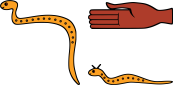
\includegraphics[scale=0.5]{word-images/1-1-4-Ddf} \\
	\hline \\ 
	\textbf{m} \textbf{r} \textbf{niwt} t $\cdot$ &
	\textbf{TA} \textbf{t} $\cdot$ &
	\textbf{p} \textbf{t} \textbf{H} \textbf{Htp} t p A50 &
	\textbf{D} \textbf{d} \textbf{f}\\
	\hline \\
	\textit{imi rA\ssn{1} niwt\ssn{2}} & \textit{TAti\ssn{3}} & \textit{ptHHtp} & \textit{Dd.f} \\  
	\hline \\
	Overseer\ssn{1} of the city\ssn{2} & vizier\ssn{3} & \sname{Ptahhotep} & (he) says:   
\end{tabularx}

\vspace{7.5mm}

\begin{tabularx}{\linewidth}{cYcY}
	\includegraphics[scale=0.5]{word-images/1-2-1-ity} &
	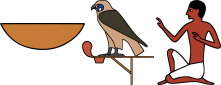
\includegraphics[scale=0.5]{word-images/1-2-2-nbi} &
	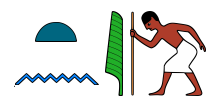
\includegraphics[scale=0.5]{word-images/1-2-3-tni} &
	
\includegraphics[scale=0.5]{word-images/1-2-4-xprw} \\
	\hline \\ 
	\textbf{it} \textbf{it} &
	\textbf{nb} G7 \textbf{A1} &
	\textbf{t} \textbf{n} \textbf{i} A19 &
	\textbf{xpr} r \\
	\hline \\
	\textit{ity} & \textit{nb.i} & \textit{tni} & \textit{xprw\ssn{4}} \\  
	\hline \\
	sovereign, & my lord, & infirmity & develops\ssn{4}
\end{tabularx}

\vspace{7.5mm}

\begin{tabularx}{\linewidth}{ccY}
	\includegraphics[scale=0.5]{word-images/1-3-1-iAw} &
	
\includegraphics[scale=0.5]{word-images/1-3-2-hAw} &
	\includegraphics[scale=0.5]{word-images/1-3-3-wgg} \\
	\hline \\ 
	\textbf{i} \textbf{A} \textbf{w} A19 &
	\textbf{h} \textbf{A} \textbf{w} D54 &
	\textbf{w} \textbf{g} \textbf{g} wr\ssn{5} D54 \\
	\hline \\ 
	\textit{iAw} & \textit{hAw} & \textit{wgg} \\
	\hline \\ 
	\indexed{old age} & befalls, & feebleness
\end{tabularx}

\vspace{7.5mm}

\begin{tabularx}{\linewidth}{cYcY}
	\includegraphics[scale=0.5]{word-images/1-4-1-iww} &
	\includegraphics[scale=0.5]{word-images/1-4-2-iHw} &
	\includegraphics[scale=0.5]{word-images/1-4-3-Hr} &
	\includegraphics[scale=0.5]{word-images/1-4-4-mAw} \\
	\hline \\ 
	\textbf{w} \textbf{i} \ssn{6} &
	\textbf{i} \textbf{H} \textbf{w} wr\ssn{5} &
	\textbf{Hr} $\cdot$ &
	\textbf{mA} A \textbf{w} Y1A \\
	\hline \\ 
	\textit{iw\ssn{7}.w} & \textit{iHw} & \textit{Hr} & \textit{mAw} \\
	\hline \\ 
	comes, & weakness & is & renewed
\end{tabularx}

\vspace*{\fill}

\pagebreak

\vspace*{\fill}

\sname{Ptahhotep} continues to lament his \indexed{old age}, describing and analogising his difficulties.

\vspace*{\fill}

8 - this appears to be a spelling mistake in the original.

9 - literally "all suns", \textit{rA} meaning "sun" and \textit{nb} used as a suffix meaning "all". \textit{rA} is identical in spelling and form to the name of the sun god \nname{Ra}.

10 - the \textit{-ti} and \textit{-wi} endings signify \indexed{dual}s, which are here translated by saying "both", whereas in English one might say "the eyes" or "the ears". In the original hieratic the singular signs are duplicated to convey the dual, and so the transcription here does the same.

11 - \textit{\indexed{ib}} is directly translated as heart, but the ancient Egyptians considered the heart to be the seat of intelligence and decision making, much as we today think about the brain.

12 - the word \textit{r} seems to be used for both the mouth and for speech.

13 - speech is only implied, this construct seems to mean something more like the colloquial or artifical english construct "wording" or "to do words".

\vspace*{\fill}

\pagebreak

\vspace*{\fill}

\begin{tabularx}{\linewidth}{cYc}
	\includegraphics[scale=0.5]{word-images/1-5-1-sDrnf} &
	\includegraphics[scale=0.5]{word-images/1-5-2-Xrdw} &
	\includegraphics[scale=0.5]{word-images/1-5-3-rA-nb} \\
	\hline \\ 
	\textbf{s} \textbf{Dr} r A55 \textbf{n} \textbf{f} &
	\textbf{X} \textbf{d} \textbf{r} wr \ssn{8} &
	\textbf{r} \textbf{A} rA \textbf{nb} \\
	\hline \\ 
	\textit{sDr.n f} & \textit{Xrd.w} & \textit{rA nb} \\
	\hline \\ 
	one sleeps & like a child & every day\ssn{9}
\end{tabularx}

\vspace{7.5mm}

\begin{tabularx}{\linewidth}{cYcY}
	\includegraphics[scale=0.5]{word-images/1-6-1-irti} &
	\includegraphics[scale=0.5]{word-images/1-6-2-nDsw} &
	\includegraphics[scale=0.5]{word-images/1-6-3-Anxwi} &
	\includegraphics[scale=0.5]{word-images/1-6-4-imrw} \\
	\hline \\ 
	\textbf{ir} \textbf{ir} &
	\textbf{n} \textbf{D} \textbf{s} \textbf{W} wr &
	\textbf{Anx} \textbf{Anx} sDm sDm &
	\textbf{i} \textbf{mr} \textbf{w} sDm \\
	\hline \\ 
	\textit{irti} & \textit{nDs.w} & \textit{Anxwi} & \textit{imr.w} \\
	\hline \\ 
	both\ssn{10} eyes & blind, & both\ssn{10} ears & deaf
\end{tabularx}

\vspace{7.5mm}

\begin{tabularx}{\linewidth}{ccYYc}
	\includegraphics[scale=0.5]{word-images/1-7-1-phtiw} &
	\includegraphics[scale=0.5]{word-images/1-4-3-Hr} &
	\includegraphics[scale=0.5]{word-images/1-7-3-aqn} &
	\includegraphics[scale=0.5]{word-images/1-7-4-wrd} &
	\includegraphics[scale=0.5]{word-images/1-7-5-ibi} \\
	\hline \\ 
	\textbf{p} \textbf{H} pHt \textbf{t} \textbf{w} A3 &
	\textbf{Hr} $\cdot$ &
	\textbf{a} \textbf{q} wr \textbf{ni} &
	\textbf{wr} r \textbf{d} A2 &
	\textbf{ib} $\cdot$ \textbf{A1} \\
	\hline \\ 
	\textit{pHtiw} & \textit{Hr} & \textit{Aq.n} & \textit{wrd} & \textit{\indexed{ib}.i} \\
	\hline \\ 
	strength & is & waning, & tired & my heart\ssn{11}
\end{tabularx}

\vspace{7.5mm}

\begin{tabularx}{\linewidth}{cccY}
	\includegraphics[scale=0.5]{word-images/1-8-1-r} &
	\includegraphics[scale=0.5]{word-images/1-8-2-grw} &
	\includegraphics[scale=0.5]{word-images/1-8-3-ni} &
	\includegraphics[scale=0.5]{word-images/1-8-4-mdwnf} \\
	\hline \\ 
	\textbf{r} $\cdot$ &
	\textbf{g} \textbf{r} A1 &
	\textbf{ni} &
	\textbf{md} d \textbf{w} A1 \textbf{n} \textbf{f} \\
	\hline \\ 
	\textit{r}\ssn{12} & \textit{gr.w} & \textit{ni} & \textit{mdw.n f} \\
	\hline \\ 
	mouth\ssn{12} & is silent, & not & speaking\ssn{13} words
\end{tabularx}

\vspace*{\fill}

\pagebreak

\vspace*{\fill}

\sname{Ptahhotep}'s lament continues.

\vspace*{\fill}

14 - this reading is uncertain.

15 - this is not an obvious translation, and the pieces referred to are not explicitly body parts. This could also be translated as places or things, although the usual word for things is \textit{xt}.

\vspace*{\fill}

\pagebreak

\vspace*{\fill}

\begin{tabularx}{\linewidth}{cYcYc}
	\includegraphics[scale=0.5]{word-images/1-9-1-ib} &
	\includegraphics[scale=0.5]{word-images/1-9-2-tmw} &
	\hspace{4mm}\includegraphics[scale=0.5]{word-images/1-8-3-ni} &
	\includegraphics[scale=0.5]{word-images/1-9-4-sXAnf} &
	\includegraphics[scale=0.5]{word-images/1-9-5-sf} \\
	\hline \\ 
	\textbf{ib} $\cdot$ &
	\textbf{tm} m \textbf{W} wr &
	\hspace{4mm}\textbf{ni} &
	\textbf{s} \textbf{X} \textbf{A} \textbf{n} \textbf{f} &
	\textbf{sf} rA \\
	\hline \\ 
	\textit{ib} & \textit{tm.w} & \hspace{4mm}\textit{ni} & \textit{sXA.n f} & \textit{sf} \\
	\hline \\ 
	heart & failing, & \hspace{3mm}not & remembering & yesterday
\end{tabularx}

\vspace{7.5mm}

\begin{tabularx}{\linewidth}{cYc}
	\includegraphics[scale=0.5]{word-images/1-A-1-qs} &
	\includegraphics[scale=0.5]{word-images/1-A-2-mnnf} &
	\includegraphics[scale=0.5]{word-images/1-A-3-Aww} \\
	\hline \\ 
	\textbf{q} \textbf{s} T19 &
	\textbf{mn} n \textbf{n} wr \textbf{f} \textbf{n} &
	\textbf{Aw} \textbf{w} Y1A \\
	\hline \\ 
	\textit{qs} & \textit{mn.n f n} & \textit{Aww}\ssn{14} \\
	\hline \\ 
	bones & hurt me from & high age\ssn{14}
\end{tabularx}

\vspace{7.5mm}

\begin{tabularx}{\linewidth}{cYccYc}
	\includegraphics[scale=0.5]{word-images/1-B-1-bw} &
	\includegraphics[scale=0.5]{word-images/1-B-2-nfr} &
	\includegraphics[scale=0.5]{word-images/1-B-3-xpr} &
	\includegraphics[scale=0.5]{word-images/1-B-4-m} &
	\includegraphics[scale=0.5]{word-images/1-B-1-bw} &
	\includegraphics[scale=0.5]{word-images/1-B-6-bin} \\
	\hline \\ 
	\textbf{b} \textbf{W} &
	\textbf{nfr} &
	\textbf{xpr} &
	\textbf{n} &
	\textbf{b} \textbf{W} &
	\textbf{b} \textbf{i} \textbf{n} wr \\
	\hline \\ 
	\textit{bw}\ssn{15} & \textit{nfr} & \textit{xpr} & \textit{m} & \textit{bw}\ssn{15} & \textit{bin} \\
	\hline \\ 
	pieces\ssn{15} & beautiful & develop & to & pieces\ssn{15} & evil
\end{tabularx}

\vspace{7.5mm}

\begin{tabularx}{\linewidth}{cYc}
	\includegraphics[scale=0.5]{word-images/1-C-1-dpt} &
	\includegraphics[scale=0.5]{word-images/1-C-2-nbt} &
	\includegraphics[scale=0.5]{word-images/1-C-3-Smti} \\
	\hline \\ 
	\textbf{d} \textbf{p} \textbf{t} ns A2 &
	\textbf{nb} \textbf{t} &
	\textbf{Sm} m \textbf{t} \textbf{i} \\
	\hline \\ 
	\textit{dpt} & \textit{nbt} & \textit{Sm.ti} \\
	\hline \\ 
	taste & all & gone
\end{tabularx}

\vspace*{\fill}

\pagebreak

\vspace*{\fill}

\sname{Ptahhotep}'s lament continues further.

\vspace*{\fill}

16 - this is a spelling mistake of \textit{ni} for \textit{n}.

\vspace*{\fill}

\pagebreak

\vspace*{\fill}

\begin{tabularx}{\linewidth}{cYcY}
	\includegraphics[scale=0.5]{word-images/1-D-1-irt} &
	\includegraphics[scale=0.5]{word-images/1-D-2-iAw} &
	\includegraphics[scale=0.5]{word-images/1-8-3-ni} &
	\includegraphics[scale=0.5]{word-images/1-D-4-rmtw} \\
	\hline \\ 
	\textbf{ir} \textbf{r} \textbf{t} &
	\textbf{i} \textbf{A} \textbf{w} A19 &
	\textbf{ni}\ssn{15} &
	\textbf{r} \textbf{t} A1 B1 Z2 \\
	\hline \\ 
	\textit{irrt} & \textit{iAw} & \textit{n} & \textit{rmtw} \\
	\hline \\ 
	what & \indexed{old age} & does to & people
\end{tabularx}

\vspace{7.5mm}

\begin{tabularx}{\linewidth}{cYcY}
	\includegraphics[scale=0.5]{word-images/1-B-6-bin} &
	\includegraphics[scale=0.5]{word-images/1-E-2-m} &
	\includegraphics[scale=0.5]{word-images/1-E-3-xtw} &
	\includegraphics[scale=0.5]{word-images/1-C-2-nbt} \\
	\hline \\ 
	\textbf{b} \textbf{i} \textbf{n} wr &
	\textbf{m} &
	\textbf{x} \textbf{t} Y1 Z2 &
	\textbf{nb} \textbf{t} \\
	\hline \\ 
	\textit{bin} & \textit{m} & \textit{xtw} & \textit{nbt} \\
	\hline \\ 
	evil & in & things & all
\end{tabularx}

\vspace*{\fill}

%\markboth{}{}

\pagebreak

\printindex

\end{document}
